\section{Hard work or celebration?}

\begin{center}
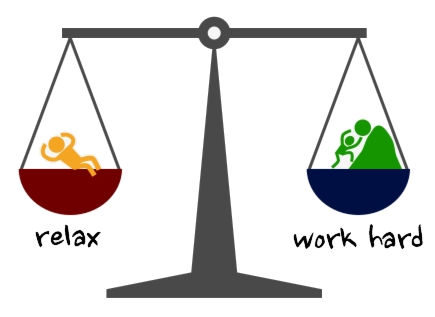
\includegraphics[width=7cm]{images/10_work.png}
\end{center}

"Well such a retreat is hard work, that can't be denied. It starts with getting up that early. Do the meditations really have to take place at 7:30 am every day? And also, why is she so peculiar about us being on time? Come on, we are not in school here! I thought we were supposed to learn to enjoy life in the now? To comply with all those rules is pretty tedious, that's more like work.

Wow, and everything is so structured: No water bottles are allowed in the room! And I am supposed to share something meaningful about me in front of all the others in the sharing circle before noon! Dancing - me?! Oh well, and then the program that lasts until late at night, are there no considerations for morning grouches?

And that was just the beginning. Then there are those exercises. To eye-gazing with total strangers, and that already at the try-out seminar. Breathe, as if there was no tomorrow. And then I am supposed to doeverything consciously... teeeedious!

It gets especially hard when we do exercises which are not that easy for me. Constantly overcoming these obstacles and motivating myself is tough work, no question."

"Hard work?! Well, only if one also refers to an adventure holiday as work.

Being on time is not a big deal as your curiosity and the excitement drive you: What might they have planned for us today? What are they going to surprise and challenge us with? Where will I learn new aspects about me? Where will I encounter limits or finally break out of an old, much too small snail house?

And the dancing! Only flying is more beautiful. Everyone on their own, all together, looks are so irrelevant! What is important is that you are allowed to show yourself, the way you are right now. Crazy, shy, stubborn, blissful. Everything is welcome. Where else do you find that?

Oh, and the sharing circles... Very impressive, touching, so much openness, vulnerability and to be given so much trust. To find oneself in the others.

In the breaks, we continue with long conversations. Deep, good talks, which bring my life on new tracks. And not to forget the touch and breath exercises. Pure bliss, timeless, vibrant energy. Unintentional, pure joy!

And by the way, the 'work' really pays off: Also my environment realizes that something is different about me, because I am simply in a better mood. I recently even spent a whole week at my parents' place. And you wouldn't believe it: They were almost unrecognizable to me!"
